\chapter{Ensayos}

\section{SBC}

\leftline{\bf{Hawkboard}}
Las Hawkboard fabricadas entre el 1º de agosto y el 20 de octubre de 2010, fueron vendidas en el mercado con un error a nivel de hardware que no había sido constatado por el fabricante, y que no fue reconocido por éste hasta el mes de noviembre. La solución al problema fue liberada en la fecha 20 de diciembre de 2010, y constaba de sustituir en el circuito los ferrites FB12 y FB13 por un puente de soldadura de estaño (el uso de jumper 0R fue probado sin obtener buenos resultados). Mayores detalles de la solución pueden encontrarse en el documento Hawkboard Press Release Solution que se adjunta en el apéndice \ref{HD}.
El inconveniente antes mencionado evitaba que el sistema operativo iniciara correctamente, en algunos casos se bloqueaba y en otros daba error en el arranque.
Esto evitó que se pudieran probar las partes de hardware y software que se tenían desarrolladas hasta ese entonces, teniendo que recurrirse a mecanismos alternativos, como el uso de un microprocesador rabbit para efectuar pruebas sobre el lector/escritor RFID.



\bigskip
\leftline{\bf{Beagleboard}}
Esta SBC no presentó problemas a nivel de hardware, por lo tanto las pruebas se basaron en verificar los cambios realizados a nivel de software.\\
Luego de la configuración de los pines del bloque de expansión a nivel de software, se realizaron las pruebas sobre las interfaces configuradas en dichos pines.

\bigskip
\leftline{Pruebas sobre las interfaces}

Testeo de GPIO: Para el testeo de los GPIO, se compiló y probó el archivo led.c (ver apéndice \ref{anx_sw_led}) el cual cambia el valor del pin 13 del bloque de expansión cada un segundo. Si se coloca un led entre este pin y nivel de referencia 0V, se puede ver como el led prende y apaga.

\bigskip
Testeo de UART: Para el testeo de la interfaz serial UART, se compiló y probó el programa uart.c
(ver apéndice \ref{anx_sw_uart}) que envía una serie de caracteres por el pin de transmisión de la interfaz UART, y luego lee por el pin de recepción de la misma el eco proveniente del pin de transmisión. Para verificar el correcto funcionamiento se deben cortocircuitar estos pines.

\bigskip
Testeo de SPI: Para el testeo del puerto SPI, se utilizó una aplicación (spidev\_test) que verifica el eco recibido cuando los pines de transmisión y recepción son cortocircuitados.\\
En este caso se debe ejecutar el archivo con los parámetros correspondientes:

\bigskip
\centerline{\$ ./spidev\_test -D /dev/spidev3.0}

spidev3.0 porque se está utilizando el puerto spi3 con chip select 0.

\bigskip
Cuando se ejecuta, deben aparecer en pantalla varias filas con “FF”. Si
se cortocircuita SIMO y SOMI algunas filas deberían cambiar, con lo que queda
verificado el buen funcionamiento del puerto SPI. \\
También se hicieron pruebas con osciloscopio, con el fin de observar la forma de las señales generadas a partir del comando:

\bigskip
\centerline{\$ ./spidev\_test -D /dev/spidev3.0 -s [Hz]}

La opción s permite configurar la frecuencia en Hz de transmisión de datos.


\section{VLT - Conversor de Voltajes}
No existieron problemas en este módulo, y dadas las características del circuito
no hay demasiados puntos de falla. Si fuera necesario verificar la diferencia de
potencial en el regulador, la tensión de entrada puede ser medida desde
el conector CONN\_14x2 y la de salida desde el conector CONN\_20x2, ver figura \ref{Fig:VLT}.
Un detalle a tener en cuenta a la hora de medir los valores de tensión de las
señales que pasan a través de los conversores de nivel, cuando las mismas se 
encuentren en estado ocioso (estáticas), es que no debe hacerse con multímetros 
de mala calidad, o se obtendrán valores incorrectos durante la medición. Se 
recomienda para una correcta medición el empleo de osciloscopio con puntas x10. 
Como se mencionó antes no se tuvieron inconvenientes con este módulo, pero generó 
conflictos en el circuito conversor full a half duplex del lector de tarjetas de 
contacto que serán detallados más adelante.


\section{SCUI - Lector de tarjetas de contacto e Interfaz de usuario}

\leftline{\bf{Lector de tarjetas de contacto ISO7816}}

Las primeras pruebas realizadas sobre el lector de tarjetas de contacto se efectuaron sobre una
placa de circuito impreso de fabricación propia, conectándose el lector directamente sobre el 
conector de expansión de la Beagleboard. La intención de esta prueba era más que nada la de probar
el circuito conversor full a half duplex, transmitiendo una serie de bytes por el canal Tx y recibiendo
el eco mediante el canal Rx, cotejando que los bytes recibidos coincidieran con los transmitidos. 
El primer problema encontrado estuvo asociado a una falla en uno de los transistores, el PNP 3906, 
que debió ser sustituido por encontrarse defectuoso.
El software utilizado para efectuar las pruebas sobre el hardware se basa en un controlador serial 
desarrollado por el grupo mina del INCO \cite{mina}, el cual fue modificado ya que uno de los parámetros, CSIZE, en la configuración del puerto afectaba el número de bits que conforman un byte recibido. 
La línea de código que hacía referencia a este parámetro fue comentada ya que modificaba el valor del parámetro 
csN, con N=5 en lugar de N=8 (donde N es el número de bits que forman el byte). 
El cambio anterior permitió que los bytes recibidos en el canal Rx coinicidieran con los transmitidos en Tx, 
validando en una primera instancia el hardware conversor full a half duplex del lector de tarjetas.
El siguiente paso fue intercalar entre la Beagleboard y el lector de tarjetas de contacto, el conversor de niveles (VLT) para realizar las mismas pruebas que se datallaron antes. En este caso los resultados no fueron alentadores ya que los bytes recibidos no coincidían con los transmitidos. Todo indicaba que el conversor de nivel afectaba el conversor full a half duplex. Luego de algunas pruebas más sobre el circuito, sin cambios favorables, se decidió consultar al foro de Texas Instruments (fabricante del integrado TXB0108). Desde el soporte técnico solicitaron se les enviara una imagen capturada con osciloscopio de las señales en el puerto serial para observar la forma de los pulsos. En la figura \ref{Fig:pulsosRx}, se puede ver la deformación de los pulsos en la señal Rx (canal 1 del osciloscopio) cuando el circuito contaba con un valor de 500 Ohms en la resistencia R9 (ver figura \ref{Fig:SAM}); la solución encontrada fue disminuir el valor de R9 y no aumentarlo como se había intentado anteriormente sin resultados favorables.

\begin{figure}[H]
\centering
  \begin{center}
  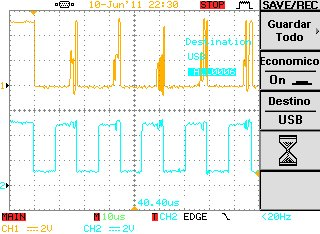
\includegraphics{Imagenes/500.jpg}
  \end{center}
  \caption{Señal en canal Rx para un valor de resistencia R9 de 500$\Omega$}\label{Fig:pulsosRx} 
\end{figure}

 Al usar valores entre 90 Ohms y 180 Ohms para la resistencia R9, la forma de los pulsos recibidos en Rx (canal 1) fueron la copia de los pulsos transmitidos en Tx (canal 2), como puede verse en la figura \ref{Fig:pulsosRx2} para un valor de 90 Ohms. 
 
\begin{figure}[H]
\centering
  \begin{center}
  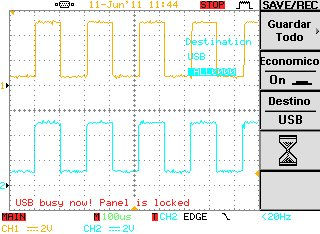
\includegraphics{Imagenes/90.jpg}
  \end{center}
  \caption{Señal en canal Rx para un valor de resistencia R9 de 90$\Omega$}\label{Fig:pulsosRx2} 
\end{figure}
 
En la siguiente referencia puede verse el hilo de discusión en el foro \cite{ForoTI}.

\bigskip
Una vez superados los obstáculos anteriores, fue posible probar el circuito completo del lector, incluyendo la tarjeta de contacto en su zócalo correspondiente. El software utilizado en tal fin se basa en un controlador serial, implementado por David Corcoran (uno de los desarrolladores de pcsclite), el cual debió ser modificado para usarse en el lector de tarjetas de contacto del prototipo RF$^{2}$. Una de las mayores dificultades encontradas en esta etapa, fue hallar los parámetros adecuados de inicialización del puerto serial, que debe cumplir con las opciones 8E2 (8 bits por byte, bit de paridad par, y dos bits de parada) para operar con las tarjetas de contacto compatibles
con la norma ISO7816. Sin embargo las opciones adecuadas elegidas en la configuración del puerto serial fueron 8E1.
Adicionalmente al problema de encontrar las opciones correctas mencionadas antes, los bytes de datos
recibidos como el ATR de la tarjeta no coincidían en su totalidad con los valores esperados (leídos con un lector Omnikey 3121 y la herramienta pcsc\_scan de pcsclite), sólo algunos bytes y algunos nibbles bajos eran correctos.
Esta diferencia estuvo asociada a la frecuencia utilizada para alimentar la señal de reloj de la tarjeta de contacto;
se usaron frecuencias de 4 MHz y 5 MHz que si bien podrían usarse según se indica en \cite{SCHb} para
los parámetros especificados en el ATR de las tarjetas empleadas, estos valores no fueron adecuados según lo ya comentado, teniendo que utilizar en su lugar un oscilador de frecuencia 3,579545 MHz, valor que no se consiguió cuando se realizó
la primer compra de componentes.
Una dificultad adicional tuvo que ser sorteada en este módulo de hardware, el diseño del PCB que se envió a fabricar
tenía un error, las pistas de datos de Rx y Tx estaban intercambiadas. El diseño tuvo que ser corregido y se 
envió a fabricar un nuevo PCB.


\bigskip
\bigskip
\leftline{\bf{Interfaz de usuario}}

En un principio, se intentó el uso de la biblioteca LCD4LINUX \cite{lcd4linux}. Éste, es un programa que se comunica directamente con el kernel para desplegar mensajes en displays con controladores como  el del display utilizado en el proyecto. Es de fácil uso y configuración, el envío de los mensajes a desplegar en el display es simple. El único inconveniente encontrado, es que la única posibilidad de configuración para el display del proyecto en el programa era por puerto paralelo. La Beagleboard no cuenta con este tipo de interfaz. Se probaron varias soluciones tratando de emular un puerto paralelo a partir de cuatro pines GPIO, pero sin grandes resultados. Se decidió reutilizar una biblioteca que el grupo de trabajo desarrolló en el marco del proyecto Audio Fingerprint del curso Procesadores Digitales de Señal \cite{Audiofingerprint}.

\bigskip
Luego, no existieron mayores inconvenientes con la interfaz para el usuario, sí fue 
necesaria la corrección en el valor de una resistencia en el circuito que calibra 
el contraste del LCD, ya que los caracteres se observaban muy tenues.

\bigskip
Al momento de probar el display imprimía caracteres extraños, salvo cuando se enviaban mensajes conteniendo una única palabra. Se probó cambiando los mensajes a desplegar en el mismo, y el problema persistía, pero se llegó a la conclusión de que era provocado por los espacios en blanco (“ ”) puesto que cuando se envió un mensaje omitiéndolos fue deplegado en forma correcta. Luego simplemente se modificó el código fuente, para que cada vez que recibiera un caracter espacio en blanco, enviara al display el caracter ASCII correspondiente solucionando el problema.

Cuando se comenzaron a imprimir los saldos de las tarjetas, volvió a imprimir caracteres extraños, esta vez el problema eran los caracteres “0” (cero). La solución encontrada fue imprimir “O” (letra o mayúscula) cada vez que llegara un caracter “0”, por lo que se modificó el código para que así sea.
Estos errores se encuentran asociados al display y no al código, que ha funcionado correctamente con otros displays.


\section{Lector/Escritor RFID}
Al comenzar la fase de pruebas sobre el lector/escritor RFID, la SBC que había sido elegida no estaba operativa por razones que ya se explicaron, y la substituta no podía ser conectada directamente al lector por incompatibilidad en los niveles de tensión que manejan sus correspondientes interfaces. Como mecanismo alternativo se usó un módulo Rabbit, RCM4300, que permitió desarrollar una pequeña aplicación de software para hacer ciertas pruebas que validaran el diseño del hardware que se tenía hasta el momento. El software implementado se basó en el estudio de la hoja de datos del integrado CL RC632, y en la biblioteca librfid \cite{librfid}. 


Una vez conectado el lector/escritor RFID al conector de expansión del microcontrolador, el paso siguiente fue configurar el puerto SPI, para esto se contó con una biblioteca provista por Dynamic C (IDE para los microcontroladores Rabbit) que permite la configuración del puerto y posee funciones para la transmisión y recepción de datos. Contar con 4 modos posibles para la configuración de este puerto del microcontrolador dificultó la tarea; fue necesario emplear un osciloscopio para observar cual de éstas se adecuaba a la forma de señal que se indica en la hoja de datos del integrado  CL RC632. Una vez seleccionado el modo correcto se pudo obtener una lectura válida del valor por defecto de los registros de página 0 del CL RC632 luego de una inicialización, no así la de registros que se encuentran en otras páginas (ver \ref{Registros} Registros), para alcanzar los demás registros fue necesario implementar una función que configurase el integrado para obtener direccionamiento plano de los registros y no por páginas.
Validada la comunicación microcontrolador - CL RC632, lo siguiente fue implementar un conjunto de funciones que permitieran la lectura/escritura de registros de control, el buffer de datos, la memoria EEPROM, el establecimiento y borrado de bits de configuración, así como también se escribieron las funciones para generar el formato adecuado de las claves de autenticación y su posterior almacenamiento en memoria. 
Cuando se culminaron las pruebas sobre el módulo digital del  CL RC632, lo próximo fue poner en funcionamiento el transmisor para establecer una comunicación con las tarjetas RFID, esta etapa fue la más compleja y que se prolongó por mayor tiempo, pues se cayó en la disyuntiva si la imposibilidad en la comunicación por RF se debía a un error cometido a nivel de hardware o de software. Por un lado se podía pensar que al seguir las pautas de diseño y los cálculos indicados en \cite{MRICF} el error no debía ser de hardware, pero a medida que los cambios a nivel de software no generaban resultados favorables, la balanza se inclinó hacia el lado del hardware. Cuando no se tiene al alcance el instrumental adecuado, un elemento que fue de mucha utilidad a la hora de comprobar la existencia de campo magnético fue un detector de campo magnético fabricado a partir de un alambre de cobre al que se le dio forma de bobina y se le soldó un led en sus extremos (ver figura \ref{Fig:detector}). Esta simple herramienta indica la presencia de campo magnético generado en las proximidades de la antena al encender su led; no olvidemos que debajo de la complejidad que puede llegar a tener este tipo de lector/escritor RFID se encuentran los principios básicos de la ley de Faraday. 


\begin{figure}[H]
\centering
  \begin{center}
  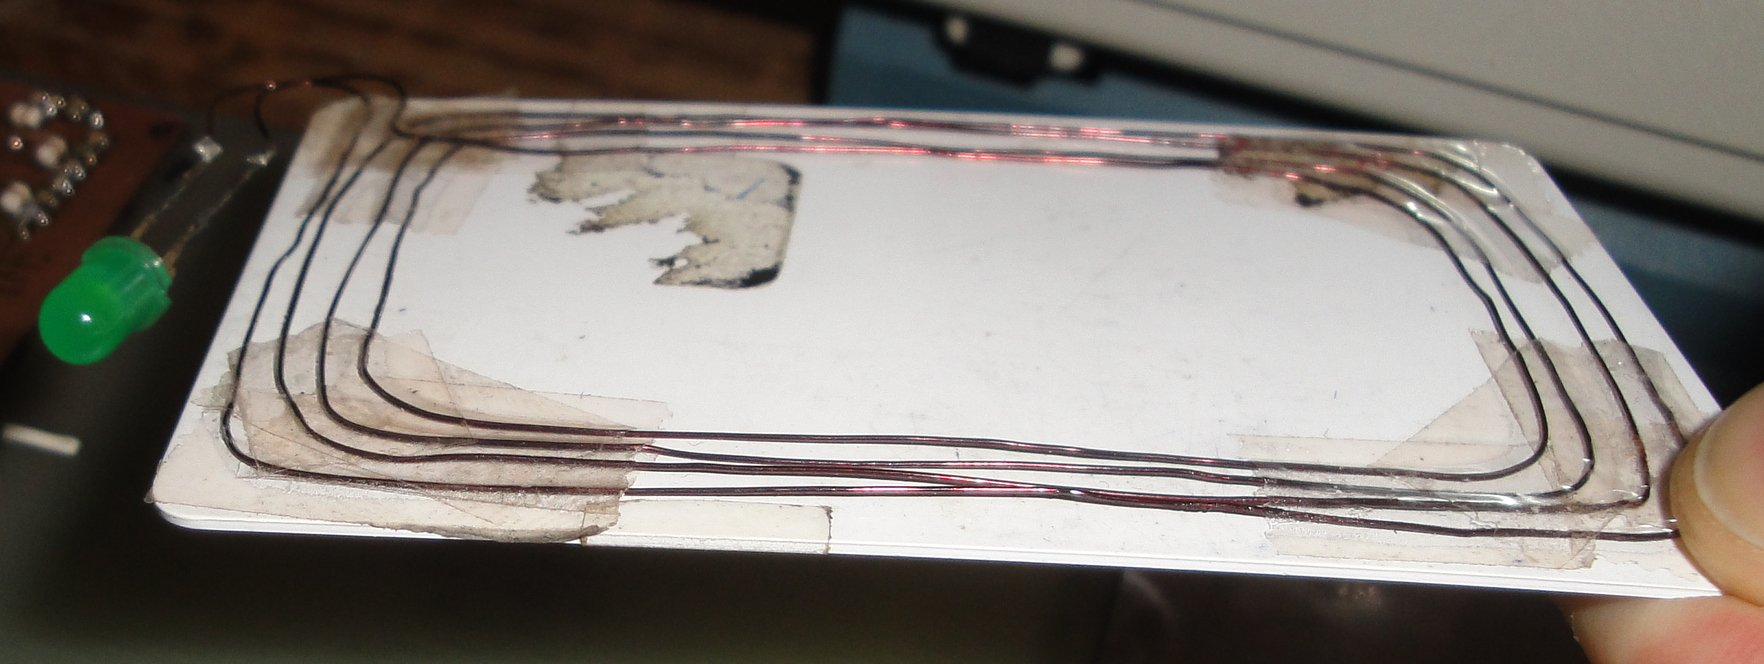
\includegraphics[scale=.1]{Imagenes/detector.jpg}
  \end{center}
  \caption{Detector de campo magnético casero}\label{Fig:detector} 
\end{figure}


Posteriores pruebas usando un osciloscopio en el que una de sus puntas de prueba formaba una espira en lazo cerrado con su línea de tierra, permitió llegar a la misma conclusión que con el detector mencionado antes, no se producía campo magnético en el entorno próximo al inductor de la antena.  
Una manera poco elegante, pero ingeniosa, de resolver el problema anterior fue desconectar el inductor fabricado en el PCB y colocar en su lugar una bobina de 3 espiras y aproximadamente 10cm de diámetro (ver figura \ref{ant_rulo}), hecha a partir de alambre de cobre con aislante incluido. La fabricación de esta bobina se basó en una similar que se puede encontrar en el lector/escritor Proxmark \cite{Proxmark} (ver apéndice \ref{HD}). 

\begin{figure}[H]
\centering
  \begin{center}
  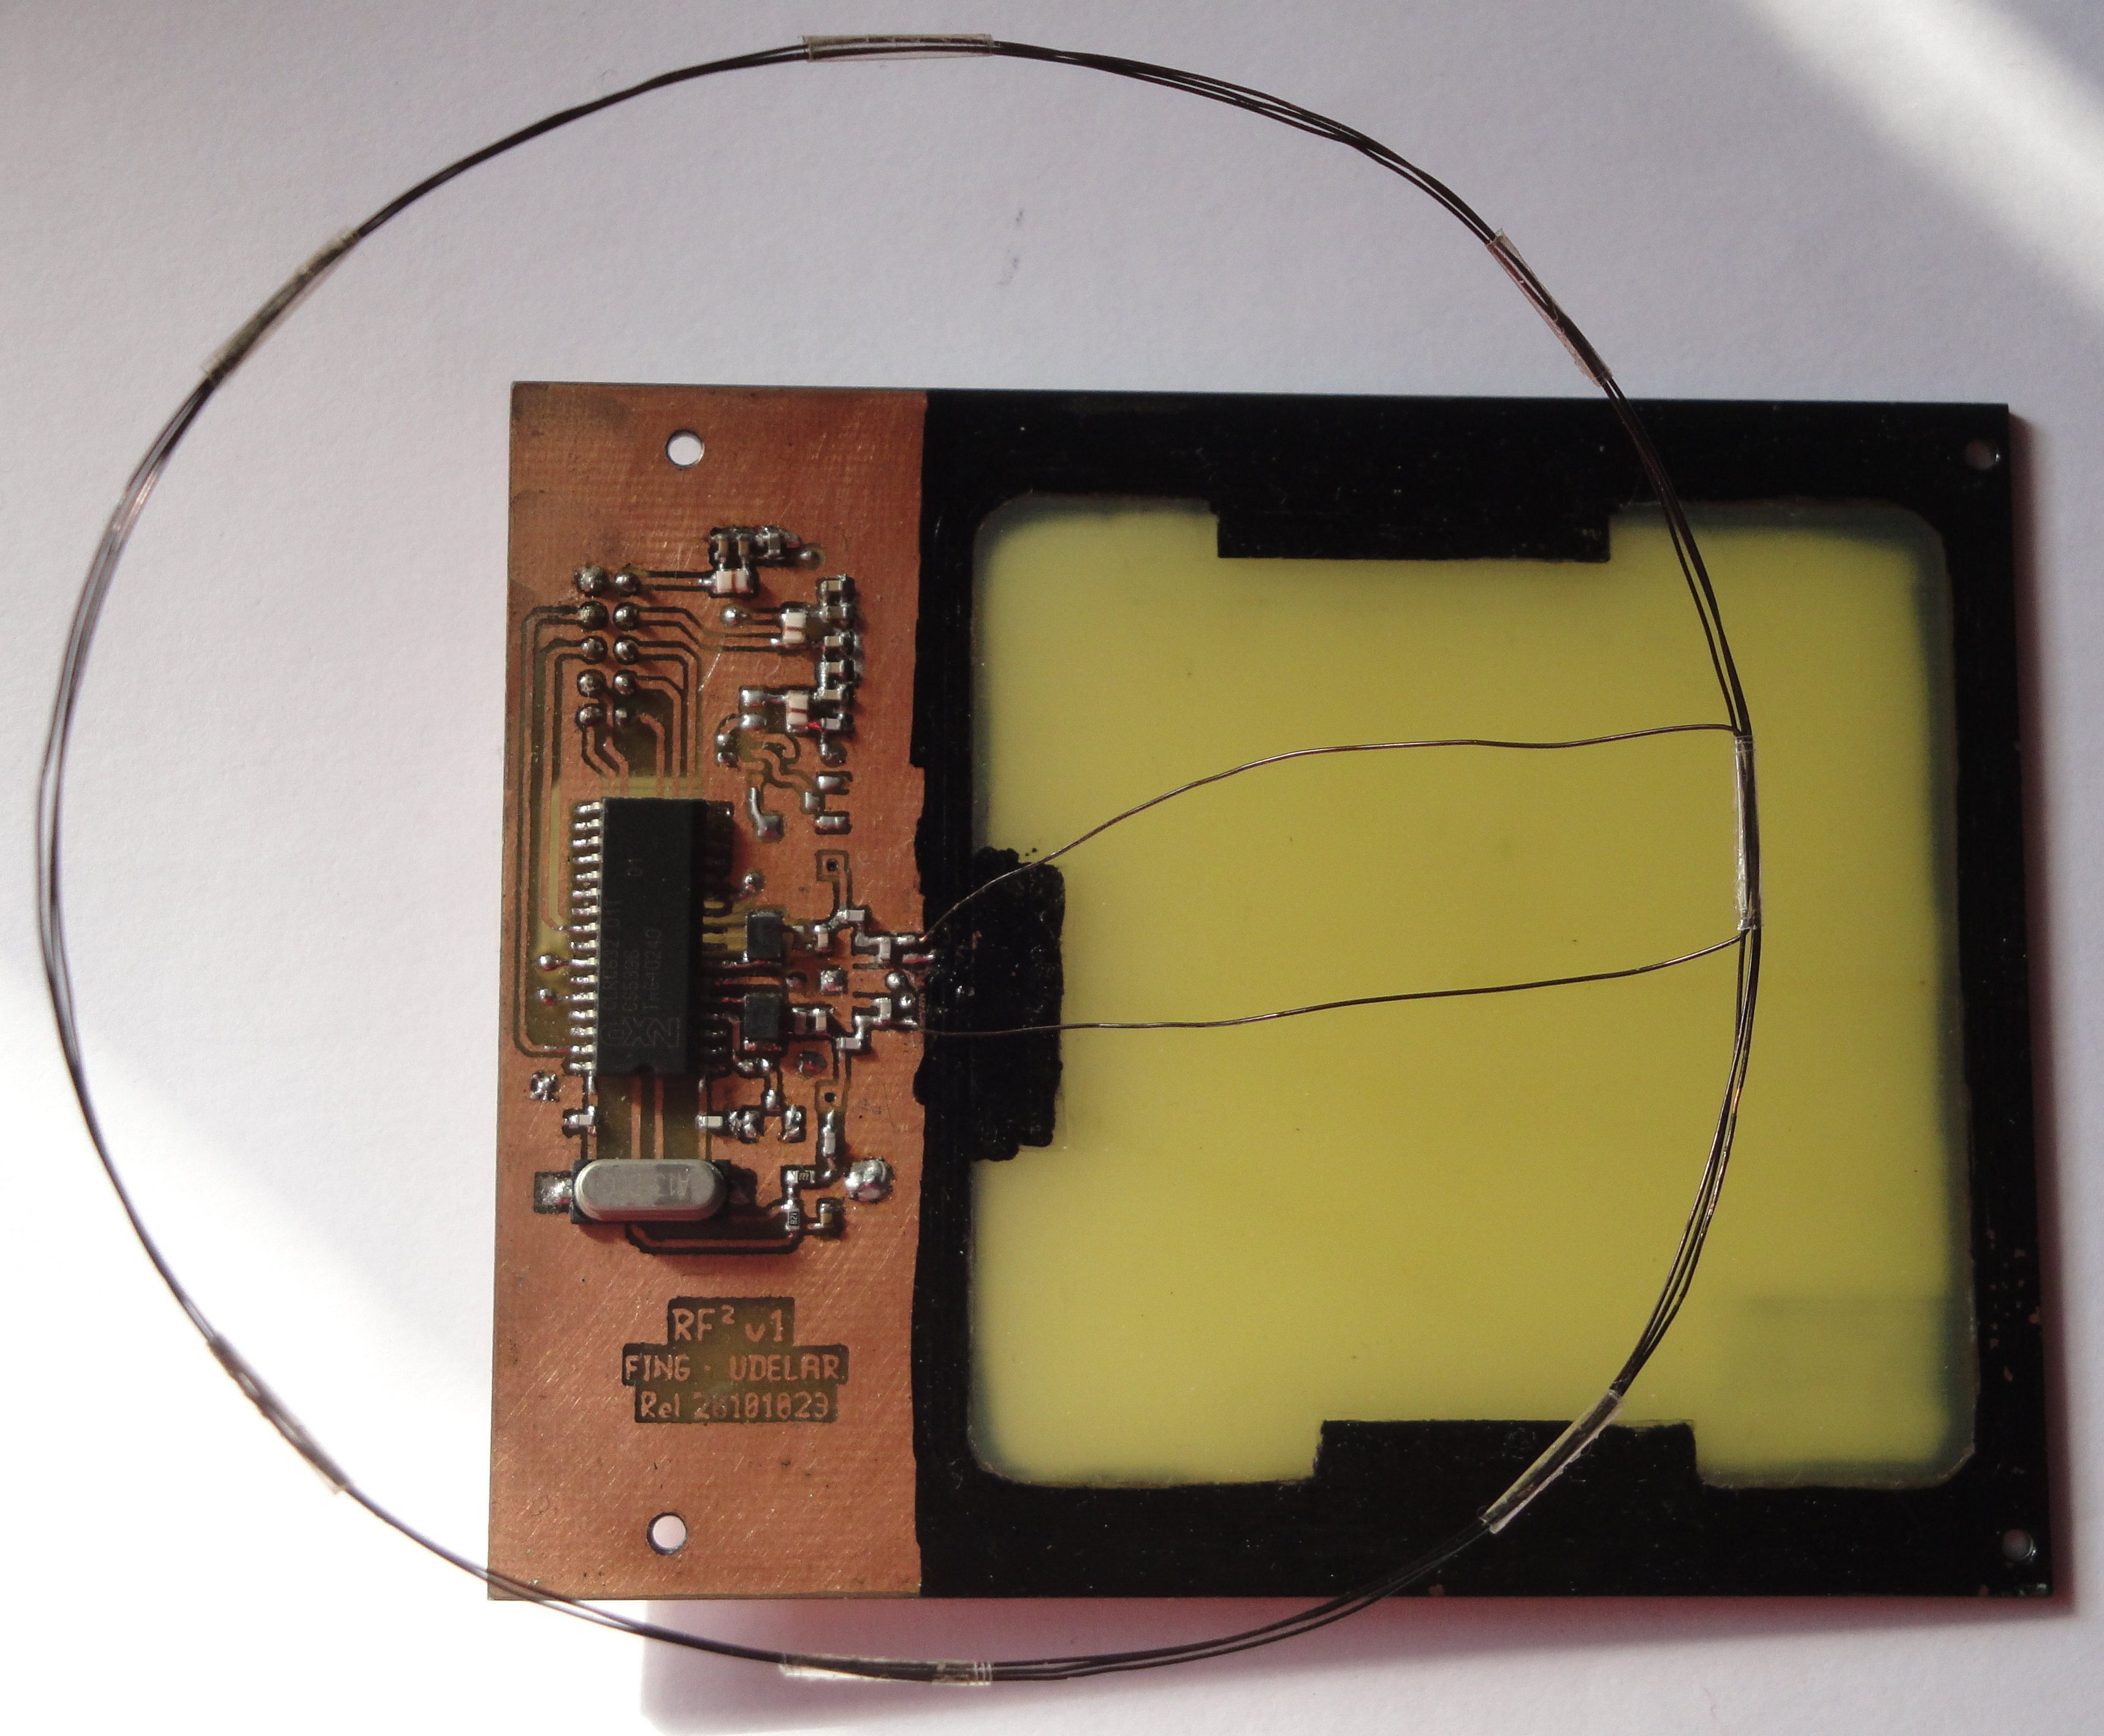
\includegraphics[scale=.1]{Imagenes/ant_rulo.jpg}
  \end{center}
  \caption{Lector/escritor RFID con bobina}\label{ant_rulo} 
\end{figure}

Este cambio permitió que la antena resonara a la frecuencia adecuada propagando la señal portadora a 13,56 MHz, siendo posible observar ésta en el osciloscopio además de poder visualizar la forma de los pulsos que se generan en la transmisión de datos desde la antena hacia una tarjeta.\\
Si se observa la figura \ref{modul}, puede verse en el canal 1 la señal portadora modulada, y en el canal 2 la señal moduladora.

\begin{figure}[H]
\centering
  \begin{center}
  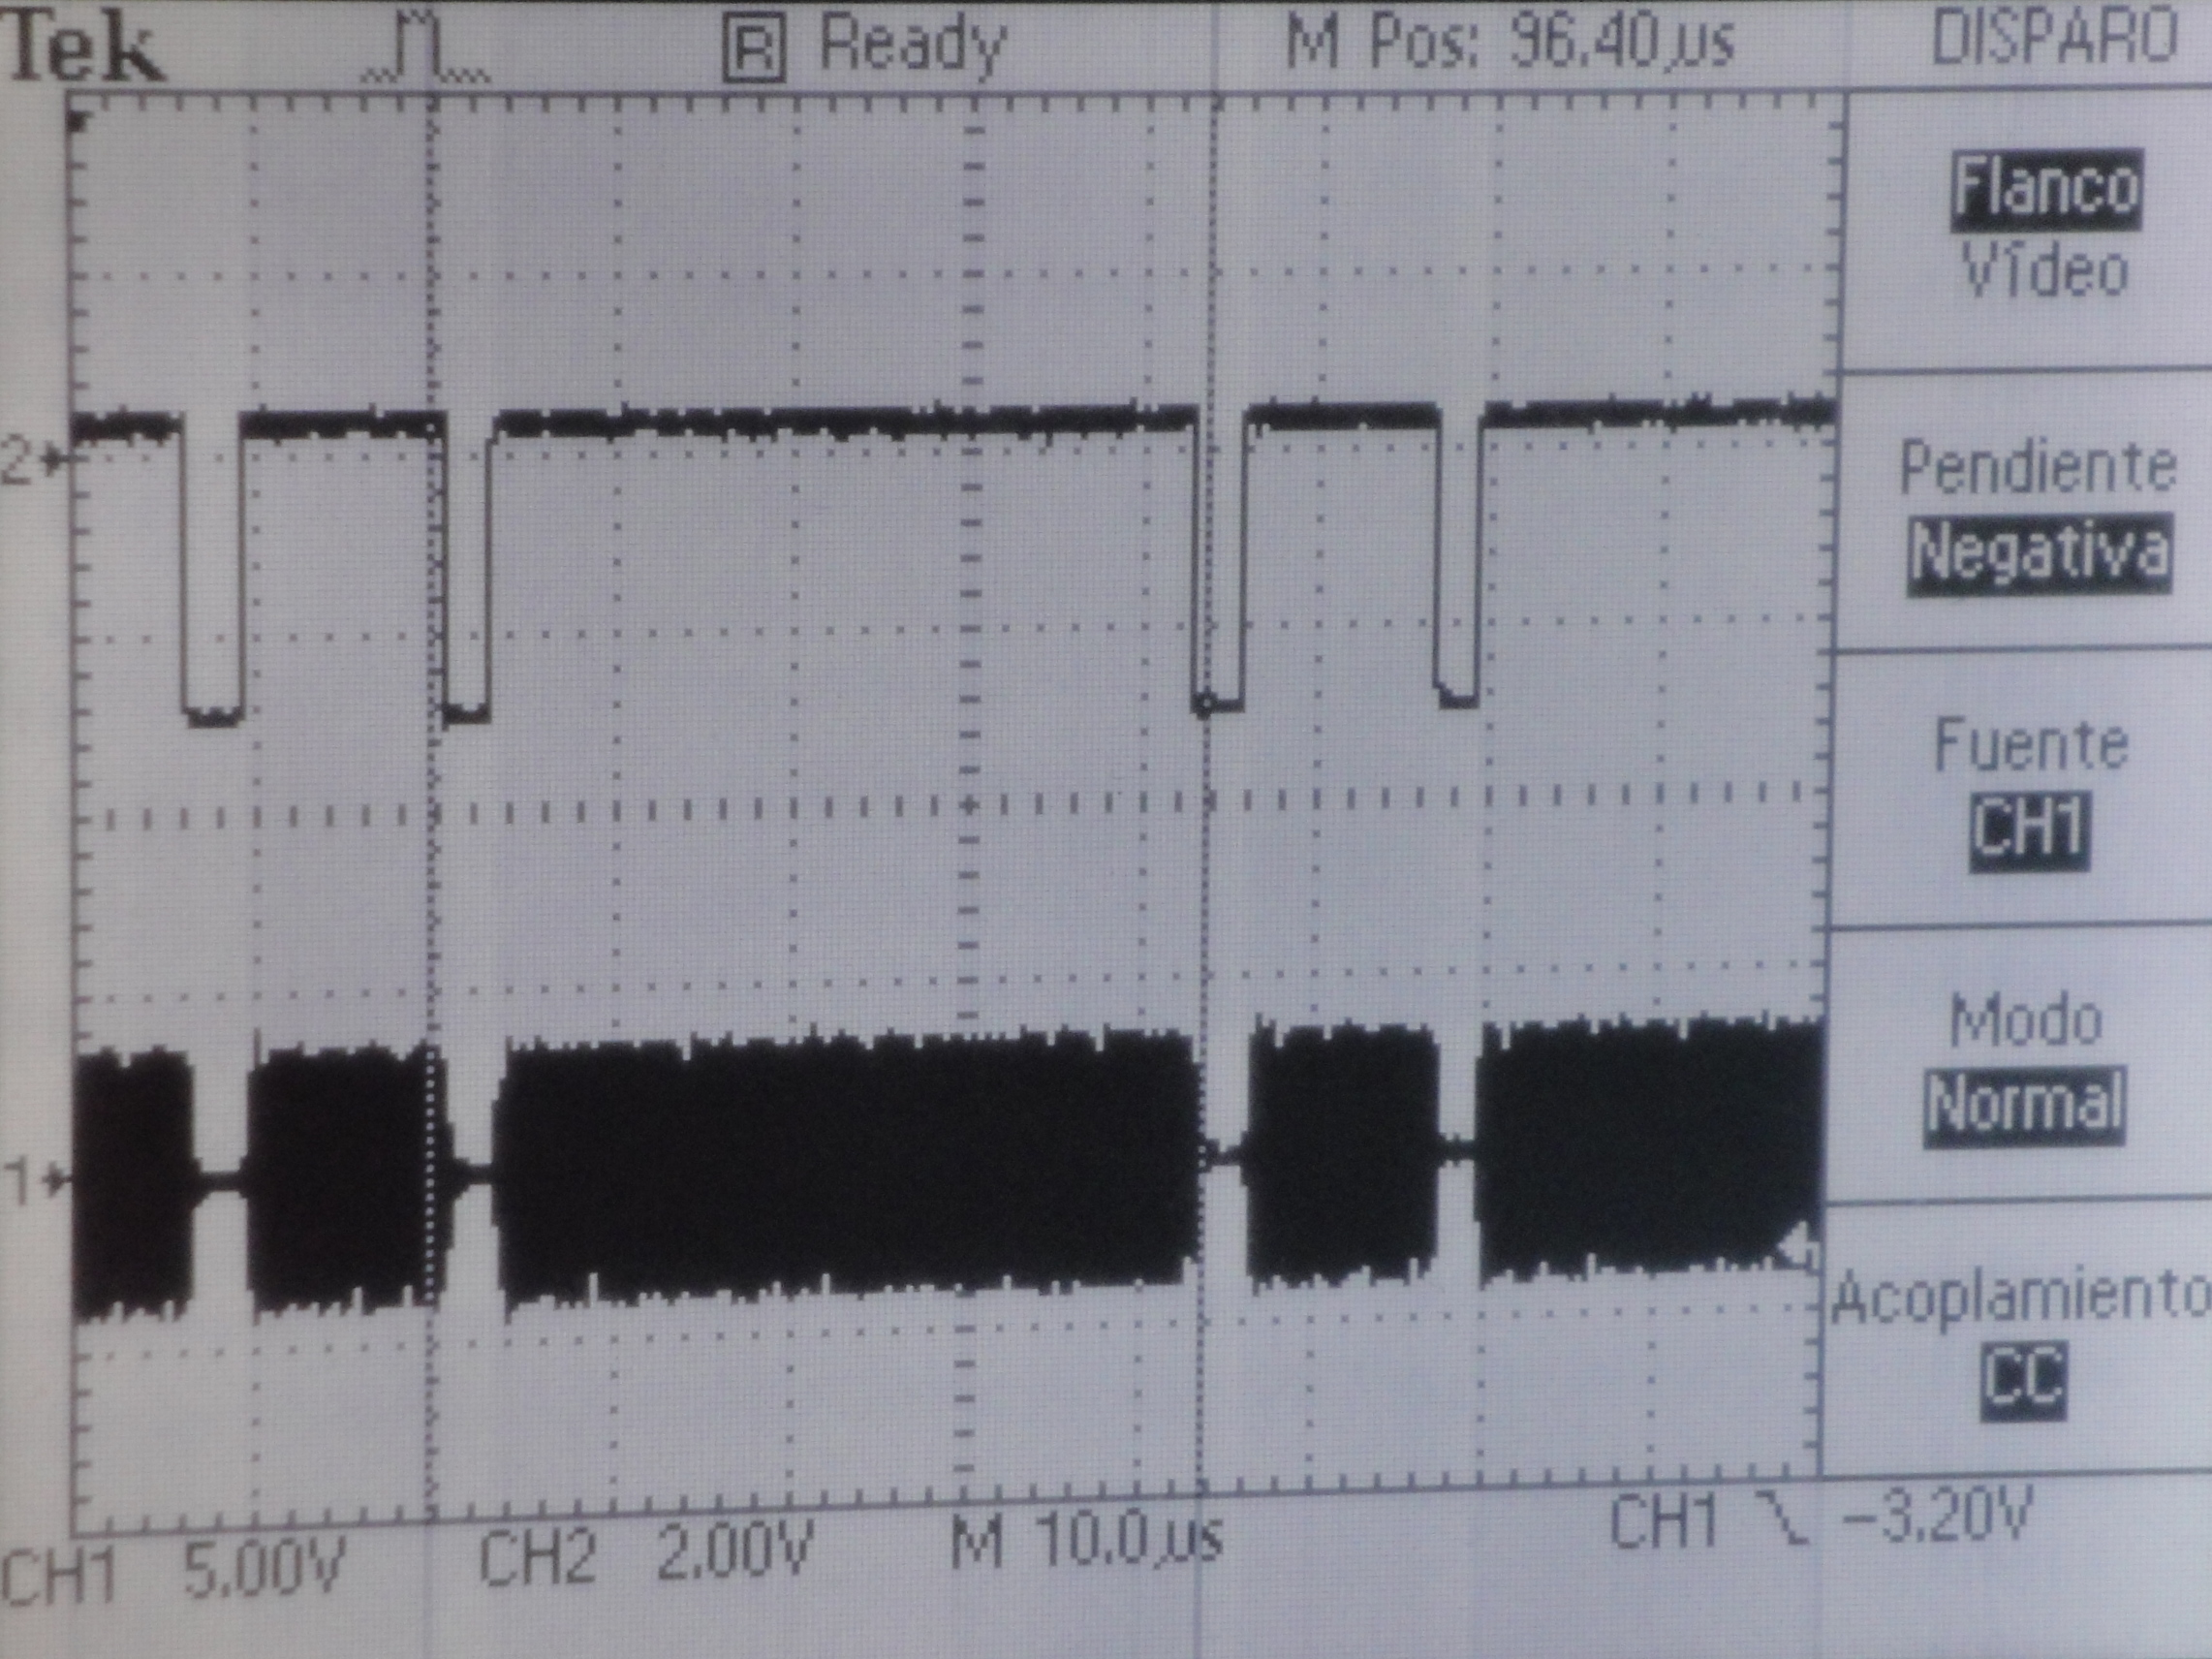
\includegraphics[scale=.2]{Imagenes/modulada.JPG}
  \end{center}
  \caption{Portadora modulada (canal 1) y señal moduladora (canal 2)}\label{modul} 
\end{figure}

Ya sin la incertidumbre a nivel de hardware, era necesario continuar con pruebas a nivel de software para lograr implementar el algoritmo de anticolisión, que permitiera obtener el UID de cada tarjeta que se aproxime al lector/escritor, así como también su autenticación y su posterior lectura y escritura. Mientras se desarrollaban las funciones necesarias, se avanzaba en paralelo en el diseño y la fabricación del conversor de niveles (VLT) que permitiera conectar el lector/escritor RFID directamente sobre la Beagleboard para hacer uso de la biblioteca librfid, que ya contaba con las funciones necesarias y simplificaría todo el desarrollo desde cero.\\
Para el testeo de la biblioteca librfid; esto es instalación, configuración y ejecución de librfid-tool; se utilizó en primera instancia un lector/escritor OpenPCD.
En las primeras pruebas se conectó el OpenPCD directo en el PC de desarrollo para luego pasar a su utilización conectado a la SBC.\\
Una vez lista la placa VLT, se conectó el lector/escritor RFID directamente sobre la Beagleboard y comenzaron las pruebas de software con la bibilioteca antes mencionada. Las primeras pruebas fueron infructíferas, decidiendo continuar en paralelo con las pruebas de software también sobre el microcontrolador Rabbit. 
Mientras se continuaba con las pruebas en software, el hardware también debía ser modificado ya que la solución alcanzada anteriormente no era definitiva sino transitoria; se resolvió entonces diseñar un nuevo lector/escritor con su módulo digital separado de la antena, esto permitiría realizar mediciones sobre ésta última haciendo uso de un analizador de red, este tipo de instrumental es sumamente útil y hasta imprescindible cuando se diseña en RF.
Las mediciones se realizaron con el instrumento: "Vector Network Analyzers" de 
ROHDE$\&$SCHWARZ (LXI Class C conformant) con que cuenta en préstamo el IIE. Por medio del mismo fue posible observar el comportamiento de la impedancia de la antena a medida que varía la frecuencia de trabajo.
Para el circuito utilizado en el primer diseño de la antena, la frecuencia de resonancia se presentaba aproximadamente a 18 MHz, es posible observar este detalle en la figura \ref{Fig:18M}. Esta frecuencia se encuentra lejos de la frecuencia de trabajo de 13,56 MHz y explica por qué no funcionaba el primer diseño.

\begin{figure}[H]
\centering
  \begin{center}
  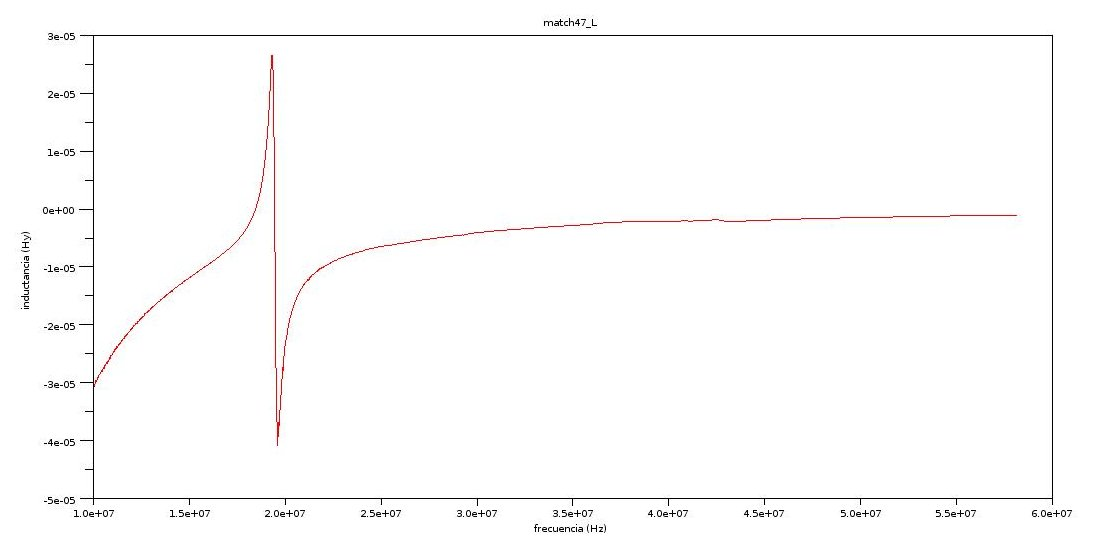
\includegraphics[scale=.45]{Imagenes/match47_L.jpg}
  \end{center}
  \caption{Módulo de impedancia z vs. frecuencia (C$_{1}$ = 10pF, C$_{2}$ = 47pF)}\label{Fig:18M} 
\end{figure}

Posteriores modificaciones en el circuito de adaptación de impedancia, incrementando o disminuyendo el valor de los capacitores según el valor de impedancia obtenida, como se indica en \cite{MRICF},  permitieron centrar la frecuencia de resonancia en 13,56 MHz como puede observarse en la figura \ref{Fig:1356M}. Se debe hacer notar que el uso de las ecuaciones para hallar los valores de los capacitores que se encuentran en las notas de aplicación \cite{MRICF} no son válidas, causando que se incurriera en error en la primer versión de la antena fabricada.  

\begin{figure}[H]
\centering
  \begin{center}
  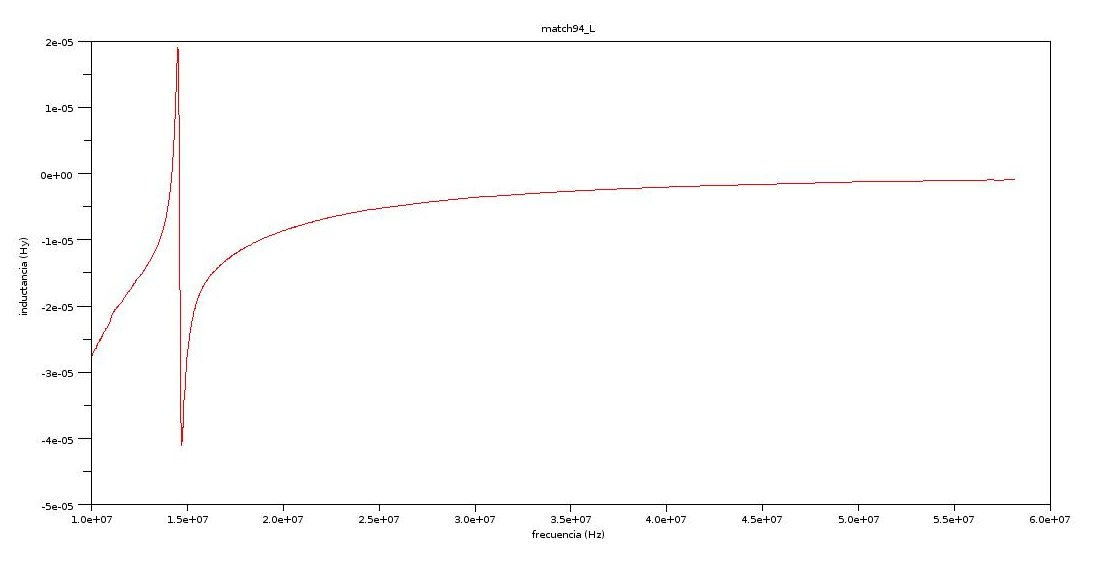
\includegraphics[scale=.45]{Imagenes/match94_L.jpg}
  \end{center}
  \caption{Módulo de impedancia z vs. frecuencia (C$_{1}$ = 10pF, C$_{2}$ = 94pF)}\label{Fig:1356M} 
\end{figure}

Las nuevas ecuaciones utilizadas se encuentran en el apéndice \ref{anx_antena}, y los valores de los capacitores que se obtienen a partir de éstas, se encuentran próximos a los obtenidos por el método práctico haciendo uso del analizador de red.
Restaba sólo incorporar el módulo digital a la antena para tener un lector/escritor RFID que permitiera continuar las pruebas de software.
Las pruebas sobre el microcontrolador Rabbit continuaron mientras no se obtenían buenos resultados usando la biblioteca librfid sobre la Beagleboard, fue posible entonces la lectura del UID que posee cada tarjeta obtenido a partir del algoritmo de anticolisión, aunque no fue posible la lectura y/o escritura de las mismas por no lograr una adecuada autenticación.
Las pruebas sobre la biblioteca librfid no arrojaron buenos resultados en una primera instancia, se tuvo que hacer algunas modificaciones, en la herramienta librfid-tool, para obtener el funcionamiento adecuado con el hardware fabricado. En primera instancia esta herramienta sólo inicializa el lector OpenPCD, sin tener en cuenta si la crosscompilación fue efectuada con opciones para manejo del puerto SPI, incorporar la inicialización del nuevo lector/escritor en esta biblioteca fue el primer paso para hacer uso adecuado del hardware. 
La siguiente dificultad que se debió enfrentar fue el haber pasado por alto que el pin RSTPD del integrado CL RC632 se encontraba en el estado lógico “1” produciendo un reset permanente, esto impedía que el integrado respondiera a las instrucciones enviadas desde la aplicación.
Resuelto lo anterior comenzaron las pruebas con la lectura de tarjetas Mifare; la lectura de un bloque de una tarjeta no ofrecía mayores inconvenientes, pero el intento de lectura completa de una tarjeta traía aparejado que no se puedieran leer sectores completos de la misma. Luego de varias pruebas en la configuración de tiempos para la transmisión de datos en el canal RF, sin buenos resultados, se probó otra opción relacionada con la tasa de transferencia de datos utilizada por librfid en el canal SPI, que se establece por defecto en el valor 1 MHz. Este valor no era adecuado para lograr una lectura completa de los 64 bloques de una tarjeta Mifare 1K, teniéndose que incrementar a una frecuencia de 10 MHz para lograr una lectura completa de una tarjeta en forma válida.
Modificaciones adicionales que no revistieron mayores dificultades fueron realizadas sobre librfid-tool con el fin de hacer uso de las tarjetas Mifare que se usan en el sistema de transporte, las que cuentan con claves de autenticación que no son las que vienen por defecto cuando las tarjetas están vírgenes. 